\documentclass[a0paper,portrait]{baposter}
\usepackage{wrapfig}
\usepackage{lmodern}
\usepackage[utf8]{inputenc} %unicode support
\usepackage[T1]{fontenc}
\selectcolormodel{cmyk}
\graphicspath{{fig/}} % Directory in which figures are stored
\newcommand{\compresslist}{%
\setlength{\itemsep}{0pt}%
\setlength{\parskip}{1pt}%
\setlength{\parsep}{0pt}%
}
\newenvironment{boenumerate}
  {\begin{enumerate}\renewcommand\labelenumi{\textbf\theenumi.}}
  {\end{enumerate}}
\begin{document}

\definecolor{darkgreen}{cmyk}{0.8,0,0.8,0.45}
\definecolor{lightgreen}{cmyk}{0.8,0,0.8,0.25}

\begin{poster}
{
grid=false,
headerborder=open, % Adds a border around the header of content boxes
colspacing=1em, % Column spacing
bgColorOne=white, % Background color for the gradient on the left side of the poster
bgColorTwo=white, % Background color for the gradient on the right side of the poster
borderColor=darkgreen, % Border color
headerColorOne=lightgreen, % Background color for the header in the content boxes (left side)
headerColorTwo=lightgreen, % Background color for the header in the content boxes (right side)
headerFontColor=white, % Text color for the header text in the content boxes
boxColorOne=white, % Background color of the content boxes
textborder=rounded, %rectangle, % Format of the border around content boxes, can be: none, bars, coils, triangles, rectangle, rounded, roundedsmall, roundedright or faded
eyecatcher=false, % Set to false for ignoring the left logo in the title and move the title left
headerheight=0.11\textheight, % Height of the header
headershape=rounded, % Specify the rounded corner in the content box headers, can be: rectangle, small-rounded, roundedright, roundedleft or rounded
headershade=plain,
headerfont=\Large\textsf, % Large, bold and sans serif font in the headers of content boxes
%textfont={\setlength{\parindent}{1.5em}}, % Uncomment for paragraph indentation
linewidth=2pt % Width of the border lines around content boxes
}
{}
%
%----------------------------------------------------------------------------------------
%	TITLE AND AUTHOR NAME
%----------------------------------------------------------------------------------------
%
{
\textsf %Sans Serif
{Brain-computer interface predicts hand motion based on cortical signals
}
} % Poster title
% {\vspace{1em} Marta Stepniewska, Pawel Siedlecki\\ % Author names
% {\small \vspace{0.7em} Department of Bioinformatics, Institute of Biochemistry and Biophysics, PAS, Warsaw, Pawinskiego 5a}} % Author email addresses
{\sf\vspace{0.2em}\\
Vadim Strijov, Anastasia Motrenko, and Roman Isachenko
\vspace{0.1em}\\
\small{ Moscow Institute of Physics and Technology --- 
Laboratory of Machine Intelligence\\
\vspace{0.2em}\\
strijov@phystech.edu}
}
{
\includegraphics[width=.22\textheight]{eng_text}} % University logo


\headerbox{Model to predict hand movement trajectories based on cortical activity}{name=introduction,column=0,row=0, span=3}{

The Brain-computer interface project aims to develop compensating systems that will help people with a severe motor control disability recover mobility. Signals are measured directly from a human brain. The predictions rely on linear models. This offloads the processor, since it requires less memory and fewer computations in comparison with neural networks. As a result, the processor can be combined with a sensor and implanted in the cranium. By simplifying the model without degrading the predictions, it becomes possible to respond to the changing brain signals. This technology could drive exoskeletons that would allow patients with impaired mobility to regain movement.
}

\headerbox{ECoG signal sources}{name=model,column=0,below=introduction,span=1}{
The implant to measure ECoG detects the electrical activity in the motor cortex with minimally-invasive implantation in the cranium and, over the long term, to measure signals thanks to an array of electrodes in contact with the dura mater~\cite{Aksenova2014ECoG}.
\begin{center}
    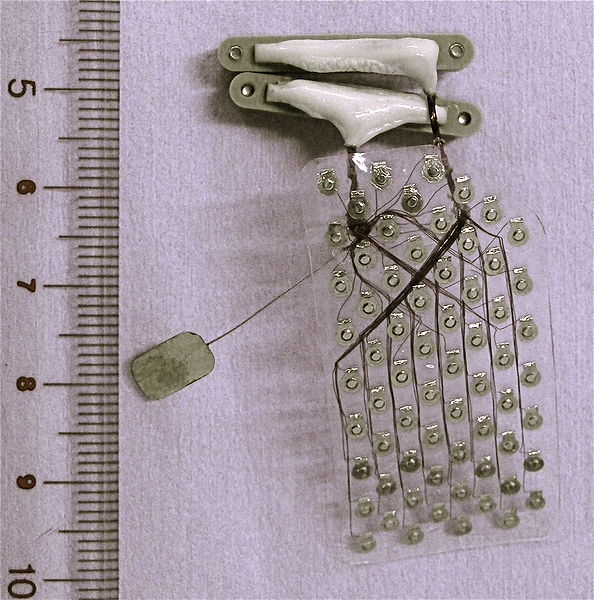
\includegraphics[width=\linewidth]{594px-CIMG0464}
\end{center}

\vspace{-0.8cm}
~~~~~~~~~~~~~~Source: neurotycho.org
}

\headerbox{Experimental setup}{name=mcs,column=0,below=model,span=1}{

The project Neurotycho aims to share reliable massive neural and behavioral data for understanding brain mechanism. The monkey was tracking food rewards with the hand contralateral to the implant side. ECoG data and motion data were recorded simultaneously during the task~\cite{Choa2010LongTerm}.% There was no eye tracking.   %“By simple I mean there are relatively few parameters. Robustness refers to the ability to retain reasonable prediction quality under minor changes of parameters. Precision means that the predictions adequately approximate natural physical limb motions. To achieve this, we predict motion trajectories as a linear combination of the electrocorticogram feature descriptions.”

\vspace{18pt}
\begin{center}
%    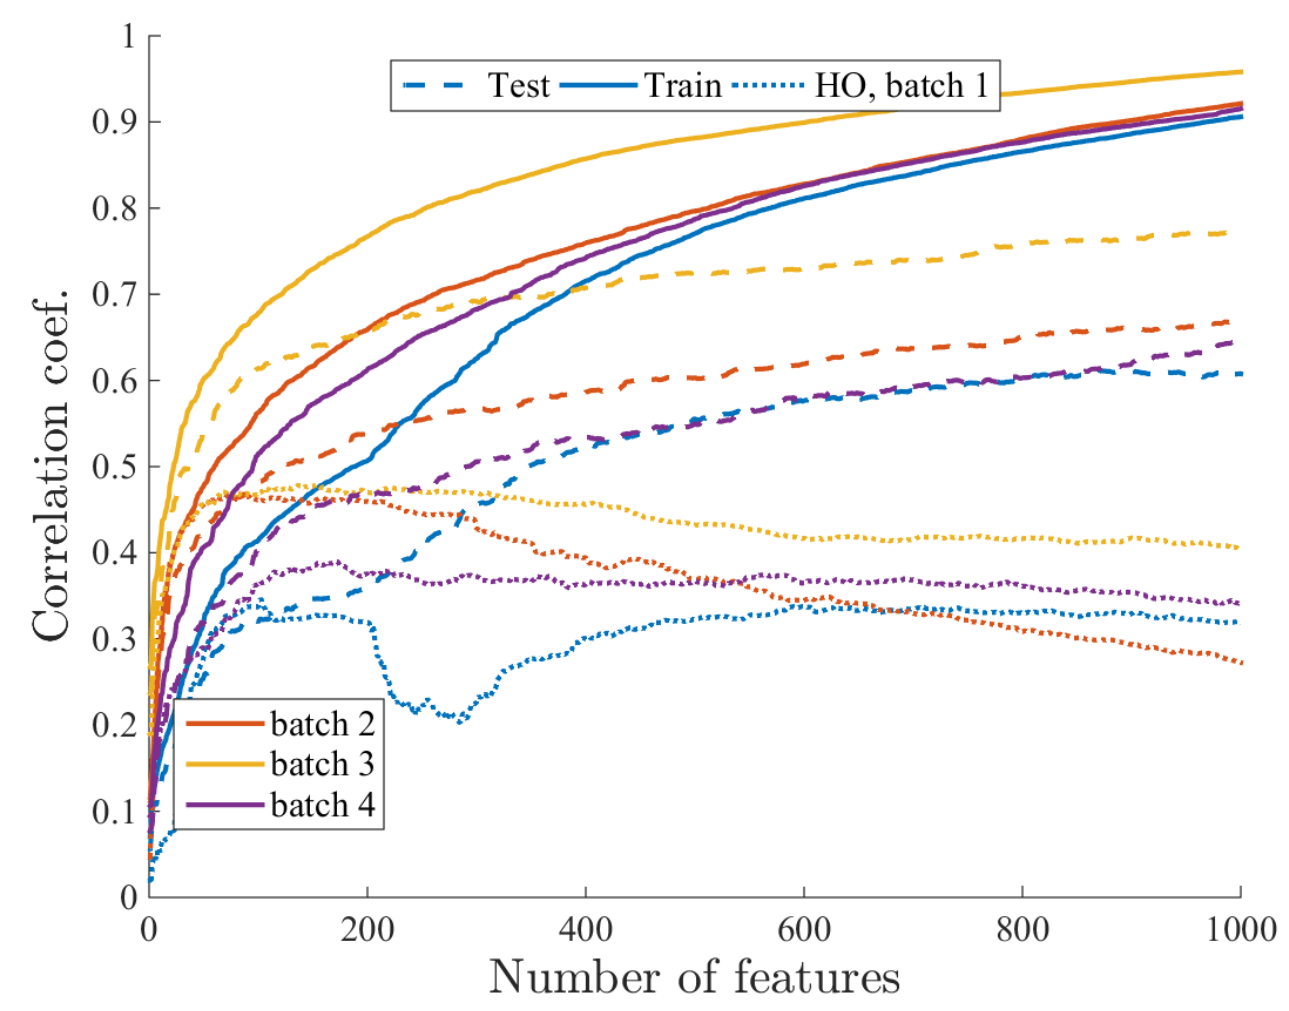
\includegraphics[width=\linewidth]{ECoGQuality.png}
    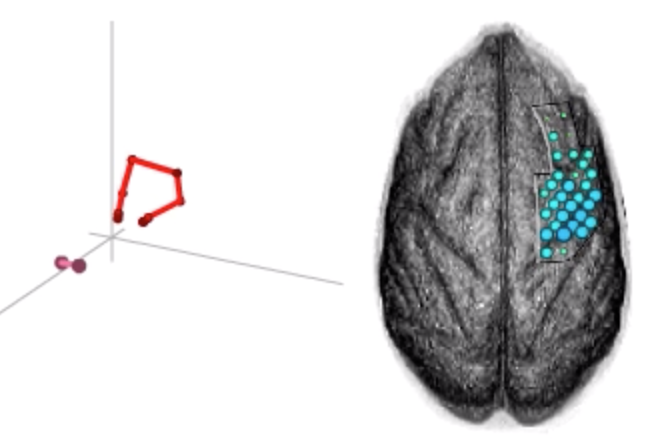
\includegraphics[width=\linewidth]{NeurotychoBrain}
\end{center}

\vspace{-1cm}
~~~~~~Source: neurotycho.org

\vspace{21pt}
ECoG and motion data were sampled at 1KHz and 120Hz, respectively, with time stamps synchronized.
}

\headerbox{Physical motion, corresponding ECoG signals, and feature representation}{name=screen,span=2,column=1,below=introduction}{ % To reduce this block to 1 column width, remove 'span=2'
 To restore motion, brain cortex signals are measured, and decoded to be transmitted to an exoskeleton. Decoding means interpreting the signals as a prediction of the desired limb motion. To pick up high-quality signals, the sensor needs to be implanted directly in the braincase. To use this data to control artificial limbs, movement trajectories need to be reconstructed from the electrocorticogram. 
\vspace{-5pt}
\begin{center}
    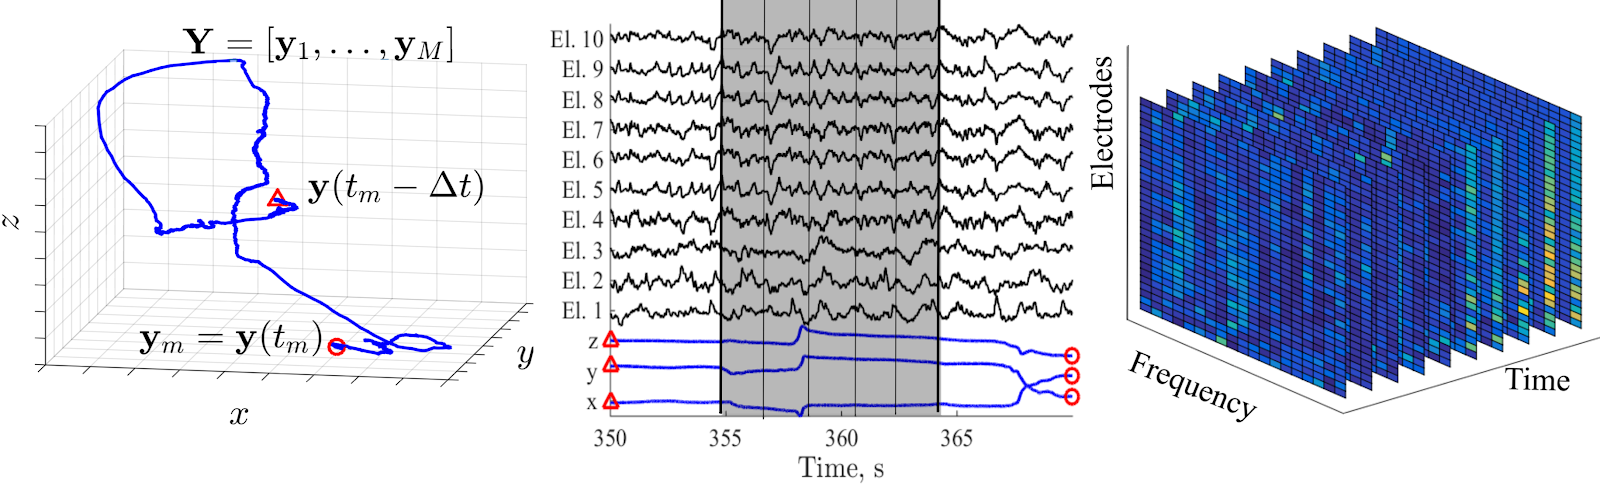
\includegraphics[width=\linewidth]{ECoGdecoding}
\end{center}
\vspace{-5pt}
{For each electrode, one-second signal intervals undergo modifications and are assigned a feature description in amplitude-frequency space. It is color-coded. The blue curve on the left is a trajectory of limb motion. Each black curve in the middle corresponds to a signal on one electrode~\cite{Motrenko2018ECoG}.}}

\headerbox{Electrodes correlate movements}{name=sea1,span=1,column=1,below=screen}{ 
 Each dot represents an electrode. The color of the dots varies between yellow and blue, indicating the similarity between the signal of the electrode and the limb motion trajectory. The trajectory is given by the three projections on the coordinate axes in the physical experiment. For each axis, there is evidently a set of electrodes suitable for reconstructing the trajectory.     
    \begin{center}
        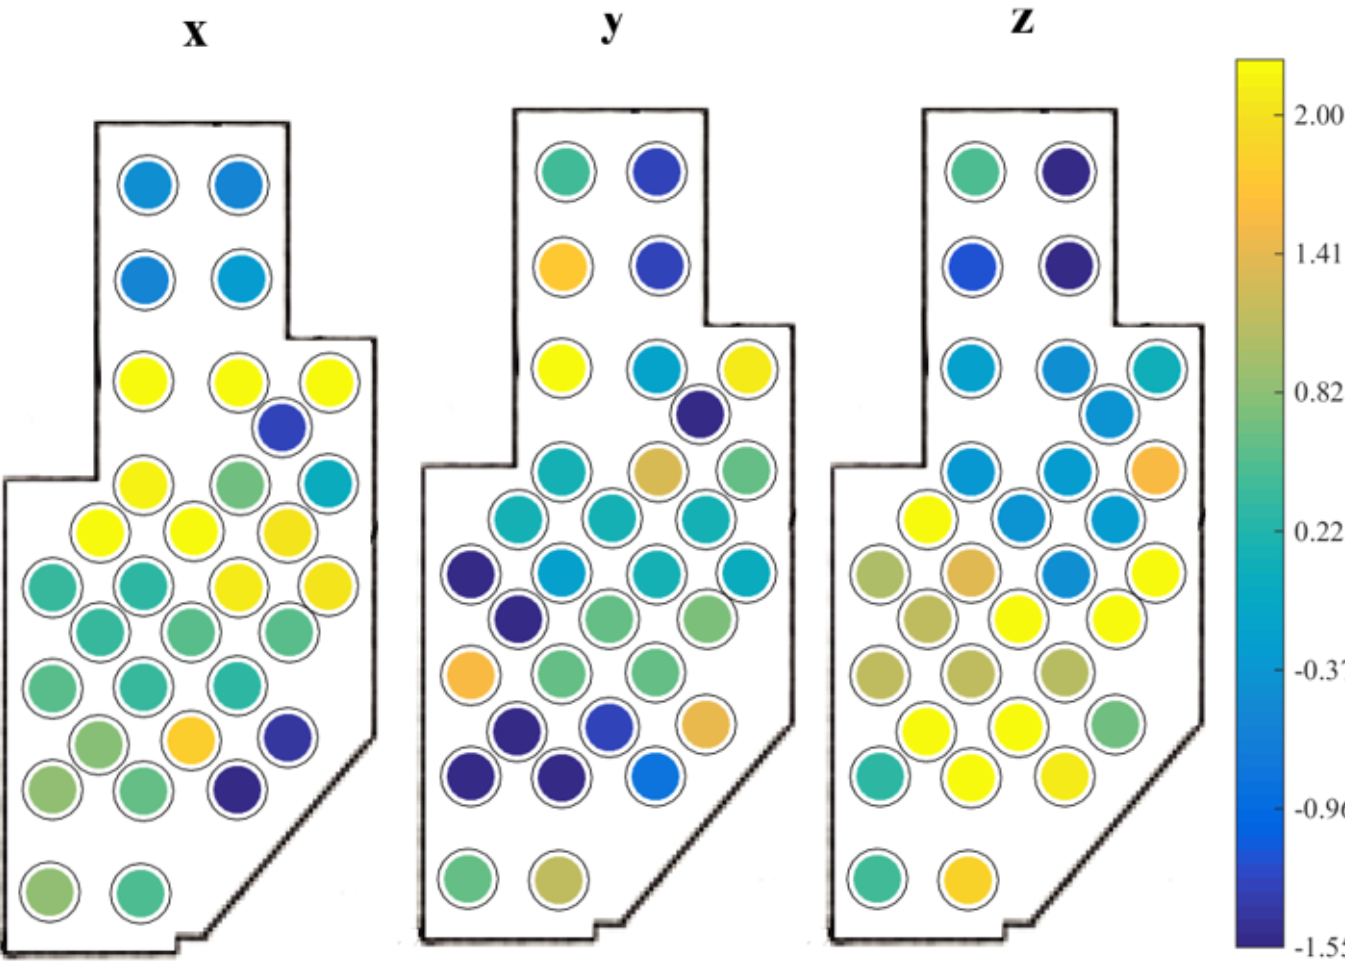
\includegraphics[width=\linewidth]{ECoGYcorr}
    \end{center}
}

\headerbox{Decoding model quality}{name=sea2,span=1,column=2,below=screen}{ The tensor model was selected to predict limb motion trajectories. The advantage of the linear models over neural networks is that the optimization of model parameters requires much fewer operations. This means they are well-suited for a slow processor with limited memory. %“By simple I mean there are relatively few parameters. Robustness refers to the ability to retain reasonable prediction quality under minor changes of parameters. Precision means that the predictions adequately approximate natural physical limb motions. To achieve this, we predict motion trajectories as a linear combination of the electrocorticogram feature descriptions.”
\begin{center}
    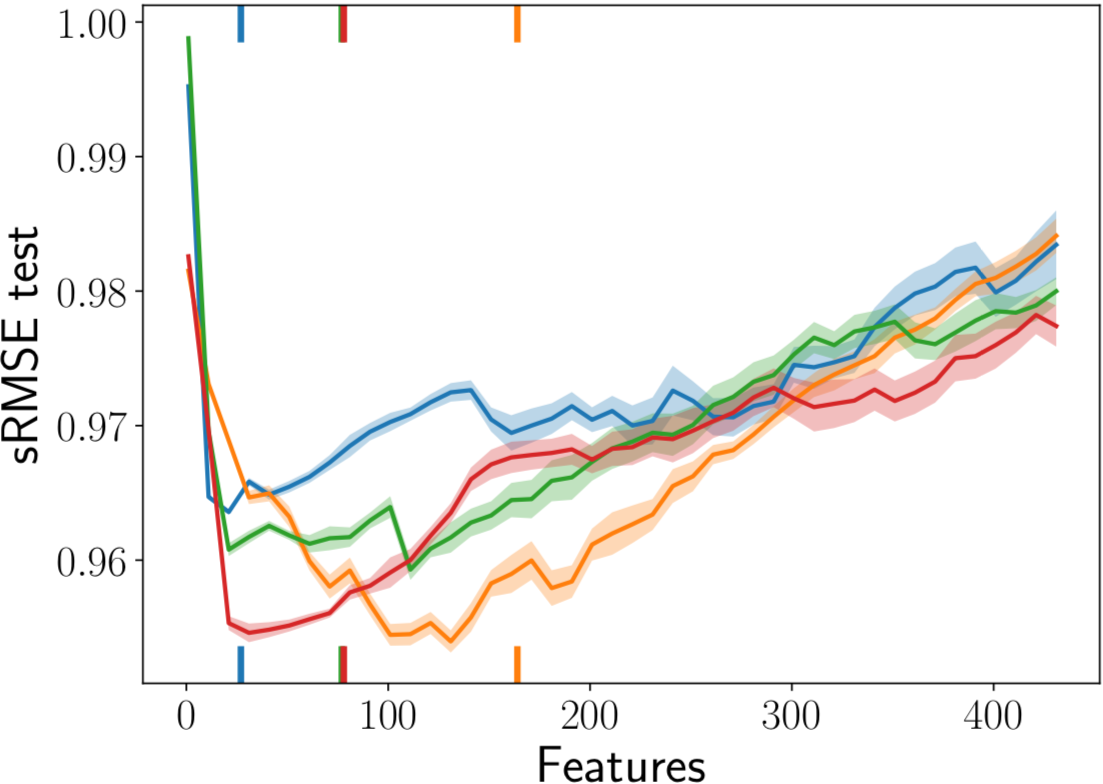
\includegraphics[width=0.86\linewidth]{ECoGRMSE}
\end{center}
The resulting model is optimized to be simple, robust, and precise with limited number of features~\cite{Isachenko2018QPFS}.
}

\headerbox{The wrist motion trajectory prediction with ECoG}{name=conclusion,column=1,below=sea1,span=2}{
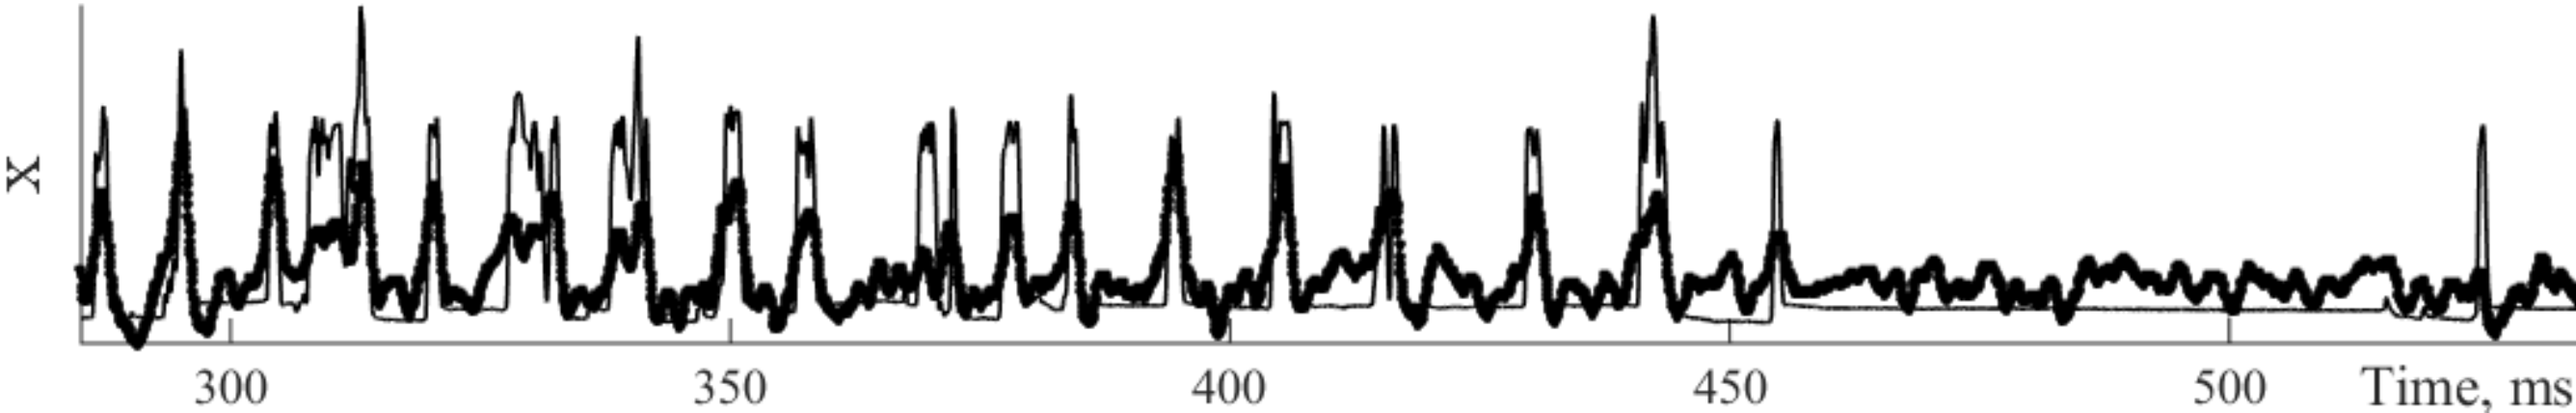
\includegraphics[width=0.95\linewidth]{ECoGPredict}
}

\headerbox{References}{name=references,column=0,span=3,below=conclusion,above=bottom}{
{\footnotesize
\renewcommand{\baselinestretch}{0.6}% Reduce the font size in this block
\renewcommand{\section}[2]{\vskip 0.05em} % Get rid of the default "References" section title
%\nocite{*} % Insert publications even if they are not cited in the poster
\bibliographystyle{unsrt}
\bibliography{Isachenko2018ECoGposter} % Use sample.bib as the bibliography file
}}
\end{poster}
\end{document}
